\documentclass{article}
\usepackage{spconf,amsmath,graphicx}
\usepackage[english]{babel}
\usepackage{color}
\usepackage{graphicx} 

\newcommand{\MARL}{Multi-Agent Reinforcement Learning}
\newcommand{\qVal}{Q-Value}

% Title.
% ------
\title{Limited Sharing Cooperative Agents in \\ Multi-Agent Reinforcement Learning}
%
% Single address.
% ---------------
\name{Meghan Day, Jake Roemer, Jeniya T Binte Jafar, Jhansi Lakshmi Kolla}
\address{The Ohio State University\\
        Department of Computer Science and Engineering\\
        %2015 Neil Ave, Columbus, OH
        }
%
\begin{document}
%
\maketitle
%
\begin{abstract}

{Demand for intelligent agents has been a large motivation in the design and implementation of enemy AI in games. Players want opponents that can act intelligently and pose a challenge. We propose MARLs, a cooperative Multi-Agent Reinforcement Q-learning approach to AI agents with limited message sharing. We believe MARLs will give the enemy agents a human-like feel which occasionally allows players to capitalize on a wrong choice that the AI makes. To evaluate the performance of this cooperative agent, we compare it against an oracle agent with unlimited message sharing and an independent agent with no message passing capacity. We found only minor improvements in performance between the different AI when limiting policy sharing between agents.
}

%{Demand for intelligent agents has been a large motivation in the design and implementation of enemy AI in games. Players want to play against enemies that can act intelligently and are also enjoyable opponents. We propose MARLs, a cooperative Multi-Agent Reinforcement Q-learning approach to AI agents with limited message sharing. We believe MARLs will give the enemy agents a human-like feel which occasionally allows players to capitalize on a ”wrong” choice that the AI makes. To evaluate the performance of this cooperative agent, we compare it against an oracle agent with unlimited message sharing and an individual agent with no message passing capacity. The evaluation shows that the oracle agent performs better than the cooperative agent and the cooperative agent performs better than the individual agent.}

%{Demand for intelligent agents has been a large motivation in the design and implementation of enemy AI in games. Players want to play against   enemies that can act intelligently and also fun to play against. We propose MARLS, a Multi-Agent Reinforcement Q-learning approach to AI agents with limited cooperative sharing. We believe MARLS will give the enemy agents a human like feel which occasionally allows players to capitalize on a "wrong" choice that AI makes. To evaluate the performance of this cooperative agent we compare it against an oracle agent with unlimited message sharing and an individual agent with zero message passing capacity. The evaluation shows that the oracle agent performs better than the cooperative agent and the cooperative agent performs better than the individual agent.}



%Players don't want to play against easy enemies who make consistently poor decisions or follows obvious patterns. Players also don't want enemies so difficult players are forced to find scenarios the AI will act unintelligibly. The intelligent agents AI design strives for are agents which act intelligently, but are fun to play against.








%Expected results should be that oracle
%outperforms the individual and limited sharing coop, because we have treated
%oracle as infinite sharing coop.
%\jake{We could also see how a single unit does
%against multiple units as an additional comparison point. So does a single unit
%against a single enemy perform generally as well as multiple units against
%multiple enemies?} 
%The limited sharing coop should vary in accuracy based on the
%amount of sharing that takes place. 
%\jake{Find the sweet spot of
%accuracy(efficiency) vs. resource passing(complexity)} Individual should be a
%lower bound compared to coop and oracle, since no information is shared between
%units.} 
\end{abstract}
%
\begin{keywords}
Q-Learning, Reinforcement Learning, Machine Learning, Exploration-Exploitation, \MARL\ (MARL) 
\end{keywords}

%


\section{Introduction}
Computer games are among the most popular applications for artificial intelligence. When developing an AI for a game, it is important to consider creating a realistic opponent, which requires that AI agents correctly capture human intelligence. Current AI techniques use oracles to simulate cooperative decisions. In a realistic environment, units might not have the same information as other friendly units. To better simulate this scenario, each unit will act as an individual and cooperate with its allies via communication.

In this paper, we propose MARLs, \MARL\ with Limited Sharing, to give a competitive yet realistic challenge to the player~\cite{Busoniu08CompSurvey}. The agents will learn independently but share information amongst their allies. In a realistic setting, two allies cannot communicate all accumulated information instantaneously, so we limit the amount of information which can be passed and between whom it can be passed per turn. This will require that the agents prioritize which information to share and with whom. We compare MARLs to an independent multi-agent that cannot share information and an oracle multi-agent with unlimited information sharing.
%who shares the full set of possible information between multi-agents per turn.

%paper organizton??

\section{Background and Related Work}
Our game is a form of Multi-Agent System (MAS), a class which emphasizes the joint action of several agents in an environment. To cooperate in MAS, AI agents can employ three types of message sharing: {\bf{1. Percepts}}, facts about the environment, such as the agent's location or intended action; {\bf{2. Events}}, a tuple representing an agent's state, action, and reward; {\bf{3. Learned policies}}, the learned utility of taking a particular action in a particular state from past experiences ~\cite{Tan93IndepVsCoop}. 

The work presented in this paper focuses on how the performance of a MAS can alter significantly with the introduction of limited message sharing. MAS can be seen in various scenarios, for example multi-agent foraging where several robots are supposed to discover particular rocks and bring them to a specific place~\cite{Panait05CooperativeMultiAgent}.


%Possibly room to extend for explination. Are we assuming the reader knows what joint action is? 

%This might be where we want to explain that we are playing Markov games where the environment is changing.

%Seems the paper should be organized: Intro -> Background (RL and MARL) -> Game Design -> Algorithms (Cooperative, Independent, Oracle)

\section{Game Description} \label{Game Description}

Our aim is to develop a board game with two teams of intelligent units to depict the importance of message sharing in an MAS. The game takes place on a two-dimensional grid of arbitrary size. The players consist of two teams with an equal number of agents, which we will refer to as units throughout the rest of the paper. The number of units scale with the size of the grid. The teams are initially placed on opposite sides of the grid using a normal distribution around a centralized point.

The game is turn based, with each team taking its turn after the other. Each unit can move and attack within a turn, in either order. All the units of a team execute their actions simultaneously. Movement is limited in direction to forwards, backwards, left, and right and in distance to a maximum movement speed scaling with the grid. Attacking is limited to units, including allies, diagonal to the current position. After attacking, the unit moves into the position formerly occupied by the defending unit, similar to the capturing movement by pawns in chess. Movement speed is determined by equation 1, where \#Rows denotes the rows of the grid and \#Columns denotes the columns of the grid. Line of sight is limited to visible squares within a radius of movement speed + 1.

\vspace{-.3 cm}

\begin{equation}\label{eqn:moveSpeed}
Move\_Speed = \frac{\#Rows + \#Columns}{10}
\end{equation}

The objective of each team is to kill all units of the opposing team. For testing, the three different types of MARL AI algorithms will play against each other. In order to handle a deadlock, where one or both teams begin to act evasively, we impose a maximum number of turns per game (default is 50) and determine the winner by score. The score of each team is determined based on equations:~\ref{eqn:score} -~\ref{eqn:ppu}.

% EQN of score
\vspace{-.5 cm}

\begin{equation}\label{eqn:score}
Score = PPU * (NU - Alive\_{EU}) - TurnPenalty 
\end{equation}

\vspace{-.4 cm}

\begin{equation}\label{eqn:ppu}
PPU = \dfrac{Total\_Starting\_Points}{NU}
\end{equation}

\vspace{-.05 cm}

$NU$ is the starting number of units per team. $Alive\_{EU}$ is the number of enemy units which are still alive and $TurnPenalty$ is the number of turns taken before the game ended.
 

 
\section{Algorithms}
\graphicspath{ {Images/} }

\subsection{Reinforcement Learning (RL)}\label{RL}
We use a reinforcement learning approach to implement three types of agents. Reinforcement learning is a type of machine learning where behavior is learned through trial-and-error interactions with the dynamic environment. Agents, or learners, determine which action to take in order to maximize  its reward. Most of the time the action with the highest expected reward is taken, which is called exploitation. Exploration is taking a new action that has not previously been taken in the same state to learn that action's utility in the current state. The exploration-exploitation trade-off is among the biggest challenge in RL. Figure-\ref{fig:res} illustrates this learning process.

%Reinforcement Learning is a form of Unsupervised Learning where agents, or learners, do not have any prior data to learn from. The learner is not told which actions to perform, but instead must discover which actions yield the highest reward by evaluating the state after performing an action. Each action is associated with a reward and based on the rewards obtained, the learner learns the best future actions to take.

 %There are two main players in any reinforcement learning
 %\begin{enumerate}
 %\item {\bf{Agent: }} learner or the decision maker~\cite{Busoniu08CompSurvey}
 %\item {\bf{Environment: }}  Things with which the agent interacts.
 %\end{enumerate}
 
 
 
 \begin{figure}[htb]

\begin{minipage}[b]{1.0\linewidth}
  \centering
  \centerline{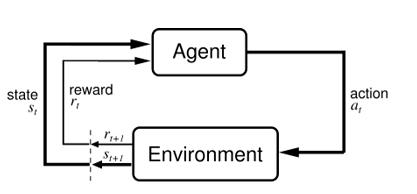
\includegraphics[width=6.5cm]{RL}}
%  \vspace{2.0cm}
  
\end{minipage}
\caption{ Agent-Environment interaction in Reinforcement Learning~\cite{Sutton98reinforcementlearning}}
\label{fig:res}
%
\end{figure}

In our case, agent is the unit of a team and state is the map of all visible units and empty positions. During each turn, the agent calculates all the possible actions in its current state and assigns an initial value to each state. This mapping is called the agent's policy. Units pick actions based on the exploration-exploitation techniques of the underlying MARL algorithms controlling each team.

A unit receives a positive reward when it kills an enemy unit and a negative reward when it is killed or kills an ally. Reward values range from [-2,1], with the highest reward for killing an enemy, 1, and the lowest rewards for killing an ally or getting killed, -1 and -2 respectively. Rewards are also given for proximity to enemy units, 0.5, and ally units, 0.25.

\subsection{\MARL\ (MARL)}\label{MARL}
We use three variants of MARL to compare the effects of message-sharing between units. In MARL, multiple agents apply RL in a shared environment and collaboratively learn a single objective. Here the policy function depends not only on the environment but also on the policies of other agents. Figure-\ref{fig:res2} explains the model of MARL.
 
\begin{figure}[htb]

\begin{minipage}[b]{1.0\linewidth}
  \centering
  \centerline{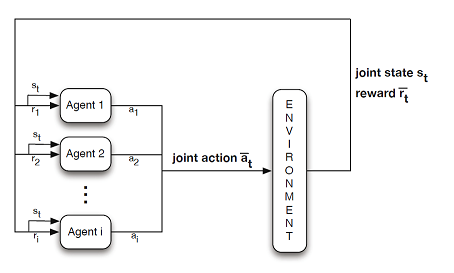
\includegraphics[width=8.5cm]{MARL}}
%  \vspace{2.0cm}
  
\end{minipage}
\caption{ Multiple agents acting in the same environment~\cite{Nowe12GameTheoryMultiAgentReinforcement}}
\label{fig:res2}
%
\end{figure}

 At each step, a joint action from all agents acts on the environment. A joint action is a vector of actions, one action per agent. The joint action acting on the environment changes the shared state and produces a reward for each agent based on the action the agent took.
 
 In our game, each team has a joint action separate from the opposing team, so at each step, one of the two teams composed of multiple agents will perform a joint action on the environment. The state will change for both teams, but the rewards for each action will only go to the agents performing the action. Then the opposing team takes a step, and steps continue until the game ends.
 
 
 
\subsection{Q-Learning}\label{QL}
Q-Learning is a Reinforcement Learning technique in which each agent keeps an individual vector of values, Q-Values, corresponding to the possible action vector for each state, so that there is exactly one \qVal\ for each state-action pair. Initially, each \qVal\ is set to -2, but once the corresponding action is taken, the \qVal\ of that state-action pair is updated based on equation \ref{eqn:q_learn}.

\vspace{- 0.5 cm}

\begin{equation}\label{eqn:q_learn}
Q(t,a) = Q(t,a) + \alpha * [r(t,a) + \gamma V(t) - Q(t,a)]
\end{equation}


%\vspace{- 0.3  cm}

Here, $Q(t, a)$ is the \qVal\ for action $a$;  $\alpha$  is the learning rate; $r(t, a)$ is the reward function which returns the reward for taking the action $a$ in the given state $t$; $V(t')$ is the value function which returns the maximum \qVal\ for the next state multiplied by $\gamma$, a scaling factor, in order to back up the highest \qVal\ from the next state.



%In our game, the set of possible actions an agent can take are all the combinations of movement and attacking for a given state. A state is defined as the relative position of visible surrounding tiles and visible agents (friend or foe).

%Most of the time an action with the highest \qVal\ is picked. Sometimes agents choose to explore an action which has not been taken earlier. By exploring an action never taken, it is possible the action results in a state yielding a higher \qVal\ which would otherwise never be taken over a high \qVal.
\section{Agent Design} \label{AgentDesign}

\subsection{Agents}

We have adopted three different MARL AI algorithms based on the amount of information shared within the Q-learning implementation~\cite{Hu98TheoreticFramework}. We use learned policy sharing in the form of Q-Value sharing for explored state-action pairs. When one unit shares Q-Values with an allied unit, the receiving unit copies the sharing unit's Q-Values for previously unencountered action-state pairs. For previously encountered action-state pairs, the receiving unit averages its current Q-Value with that of the sharing unit. Percepts and events are not shared. The first implementation is an oracle agent with unlimited sharing of Q-Values between allied units. The second is a cooperative agent with limited sharing of Q-Values. The third implementation is an independent agent with no sharing of Q-Values. 





%We have not implemented obstacles yet

%The game takes place on a two-dimensional grid of arbitrary size. The players consist of two teams of agents, which we will refer to as units throughout the rest of the paper. The number of units scale with the size of the grid. The teams are initially placed on opposite sides of the grid using a normal distribution around a centralized point.

%We did not limit movement when trying to move through a space an enemy already occupies. Units cannot move through positions occupied by obstacles or enemy units.

%The game is turn based, with each team taking its turn after the other. Each unit can move and attack within a turn, in either order. All the units of a team execute their actions simultaneously. Movement is limited in direction to forwards, backwards, left, and right and in distance to a maximum movement speed scaling with the grid. Attacking is limited to units (friend or foe) diagonal to the current position. After an attack, the attacking unit moves into the position formerly occupied by the defending unit, similar to the capturing movement by pawns in chess. How far a unit can move is determined by equation~\ref{eqn:moveSpeed}. Here, $\#Rows$ denotes the rows of the grid and $\#Columns$ denotes the columns of the grid. In addition to limiting movement, each unit's knowledge is limited to a fixed number of visible squares defined as Move\_Speed + 1.

%\vspace{-.3 cm}

%\begin{equation}\label{eqn:moveSpeed}
%Move\_Speed = \frac{\#Rows + \#Columns}{10}
%\end{equation}

%In addition to limiting movement, obstacles also limit units' line of site, preventing them from knowing what is on the opposite side. Each unit's knowledge is limited to what it can see within a 5 square radius. \\

%The objective for each team is to kill all units of the opposing team. For testing, the three different types of MARL AI algorithms will play against each other. In order to handle a draw, where units decide to stop attacking in order to keep living, MARLS imposes a maximum number of turns per game (default is $50$). If neither team can win within the turn limit, then the winner is decided by score. The score of each team is  determined based on equations:~\ref{eqn:score} -~\ref{eqn:ppu}.
%and the game will allow for a human to play against an AI or for two different AI implementations to play against each other. In order to prevent a draw condition, we will impose a maximum number of turns per game (here we choose it as $10$. When this maximum is reached, the score will be determined based on equation-~\ref{eqn:score}. Finally the winner is determined based on higher score.
%percentage of surviving units on each team and the number of steps taken per team.

% EQN of score
%\vspace{-.5 cm}

%\begin{equation}\label{eqn:score}
%Score = PPU * (NU - Alive\_{EU}) - TurnPenalty 
%\end{equation}

%\vspace{-.4 cm}

%\begin{equation}\label{eqn:ppu}
%PPU = \dfrac{Total\_Starting\_Points}{NU}
%\end{equation}

%\vspace{-.05 cm}

%Teams have the same starting size. $NU$ is the starting number of units per team. $Alive\_{EU}$ is the number of enemy units which are still alive. TurnPenalty is the number of turns taken before the game ended.

%A unit receives a positive reward when it kills an enemy unit and a negative reward when it is killed or kills an ally. Reward values range from [-1,1]. The highest reward is for killing an enemy, $1$. The lowest reward is for killing an ally or getting killed, $-0.75$. Rewards are also given for proximity to enemy units, $0.5$, and ally units, $0.25$.

%Units pick actions based on the exploration-exploitation techniques of the underlying MARL algorithms controlling each team. We have adopted three different MARL AI algorithms based on the amount of information shared within the Q-learning implementation~\cite{Hu98TheoreticFramework}. Each joint action decision for each team is determined by either the Oracle, Independent, or Cooperative algorithm using a utility function based on the current game state and set of possible actions for that state. In the following subsections we present a brief description of these three MARL AI algorithms.



%Should we explain exploration-exploration or use a different term to describe what the AI algorithms are doing?
\subsection{Oracle Agent}\label{Oracle_Agent}

The oracle agent makes decisions by using the collective experience of all of its units. During each turn, all the units calculate their individual Q-Values based on the outcome of their last state and action. Then, each unit shares this new value with all of its allied units, who copy this Q-Value if they have previously not encountered the corresponding state-action pair. Because it combines all the experience from all its units, we expect the oracle agent to perform better than the cooperative and independent agents.

%The oracle agent makes decisions by using the collective knowledge of all of its units. This agent has the knowledge of the locations of each unit and locations of the enemies which are within range of visible squares of the units. Based on all of this information, the oracle makes a decision for its next move.
 

%Because of combining all the knowledge from all its units, the oracle agent performs better than the cooperative agent. This scenario can be explained with figure-~\ref{fig:coop_vs_oracle}. %Here we consider a $3*3$ board where the visible square is $1$. Now if black circled units are controlled by the cooperative agent then unit-1 will have no knowledge of unit-2. So both will try to attack the enemy unit-A. Which ever unit kills enemy unit-A first will die by the second attacking ally unit. On the other hand if the black circled units are controlled by oracle agent then the agent will choose one unit from unit-1 and unit-2 based on their Q-values to attack unit-A
%Here we consider a $3$ by $3$ board where the visible range is $1$. Now if black circled units are controlled by the cooperative agent then unit-1 will have no knowledge of unit-2, so both will try to attack the enemy unit-A. Whichever unit kills enemy unit-A first will die by the second attacking the ally unit. On the other hand if the black circled units are controlled by oracle agent then the agent will choose either unit-1 or unit-2 based on their Q-values to attack unit-A



%\begin{figure}[htb]

%\begin{minipage}[b]{1.0\linewidth}
 % \centering
 % \centerline{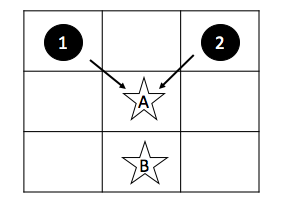
\includegraphics[width= 3.5 cm]{coop_vs_oracle}}
%  \vspace{2.0cm}
  
%\end{minipage}
%\caption{Comparing movements of oracle agent with cooperative agent}
%\label{fig:coop_vs_oracle}
%
%\end{figure}

\subsection{Cooperative Agent}\label{Coop_Agent}

The cooperative agent is implemented with limited message sharing. In our implementation, during every turn each unit shares its updated Q-Values with a subset of its allies, no greater than 3, who are selected at random. The chosen allies will share their state experience, by sharing the actions associated with the shared state. This includes sharing both unencountered action-state pairs and perviously encountered action-state pair.

Q-Values are also shared when determining the result of the Value function, which helps emphasize a good action even if a unit has not taken it yet, but an ally has. Because the cooperative agent has the ability to share some limited experience between units, we expect it to perform better than the independent agent.


%The Cooperative agent is implemented with limited message sharing. In our implementation, each unit shares information with allies, but is limited to only sharing with a set number of allies and only specifically requested information. Units of the same team are allowed to share learned experiences, or Q-Values, with each other when determining which action to take. Q-Values are also shared when determining the result of the Value function, which helps emphasize a good action even if a unit has not taken it yet, but an ally has.

%to shared experiences with each other, \qVal, when determining which action to take. \qVal\ are also shared when determining the result of the Value function which helps emphasize a good action even if a unit has not taken it yet, but an ally has.


%There are a number of types of messages sharing which AI agents can employ to cooperate. 
%Among Three types of messages \ref{background} are facts, such as the location of an enemy unit or an agent's intended action, events, including an agent's perceived environment, action taken, and result, and learned policies, such as retreating when surrounded by multiple enemy units~\cite{Tan93IndepVsCoop}. In our approach, we will employ the first of these, fact sharing. Agents will be able to share their own location and that of enemies within their range of sight with their allies.
\subsection{Independent Agent}\label{Independent_Agent}
The independent agent is implemented with no message sharing. In this implementation, each unit is controlled by itself only, so the decisions are made based only on the knowledge available to that particular unit. 


%decision by one unit = decision other unit. this may inclue friendly firing

%Due to combining partial knowledge from its units, the cooperative agent performs better than the independent agent. This scenario can be explained with figure-~\ref{fig:coop_vs_ind}. Here we consider a $3$ by $3$  board where the visible square is $1$ and the black circled units are controlled by the cooperative agent. Now unit-2 can move to the middle cell of top row, so that if unit-1 is killed by enemy unit-A then unit-2 can attack it in the next turn. The independent team has no such message passing, so unit-2 will choose its action without considering the effect on its team score. Therefore the performance of the independent agent is not as good as the cooperative agent.
%and then unit-2 will move to the middle cell of top row, so that if unit-1 is killed by enemy unit-A then unit-2 can attack it in the next turn. But independent team has no such message passing. So unit-2 will choose is action with out considering the effect on team score. Therefor the performance of independent agent is not as good as the cooperative agent.


%\begin{figure}[htb]

%\begin{minipage}[b]{1.0\linewidth}
%  \centering
%  \centerline{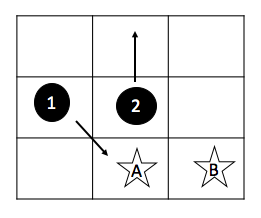
\includegraphics[width=3.5cm]{coop_vs_ind}}
%  \vspace{2.0cm}
  
%\end{minipage}
%\caption{Comparing movements of independent agent with cooperative agent}
%\label{fig:coop_vs_ind}
%
%\end{figure}

%\vspace{-.5 cm}
\section{Experiment}
% prof suggestion :: still under implementation. We are planning to do this & this. We are expecting result like this

Due to the nature of MARL and our game rules, we don't need any prior data collection. Reinforcement learning will collect data as each game is played. We have implemented a simulation of the game described in section~\ref{Game Description} along with the three different MARL AI implementations. The different MARL AI are pitted against each other over a series of games to measure how each AI learns based on the number of wins, and average score, calculated by equation~\ref{eqn:score}.

To meausre how each AI learns, we take a set window of games and evaluate the number of wins, average score, and average turns to win seperate from all other windows. For 10000 games, each window is of size 1000 games and will show the progress in learning every 1000 games. Scores are listed above wins in each graph as a difference between the two team's scores.
%High performance is indicated by higher win success rates with higher average scores and lower average turns to win.

 \begin{figure}[htb]

\begin{minipage}[b]{1.0\linewidth}
  \centering
  \centerline{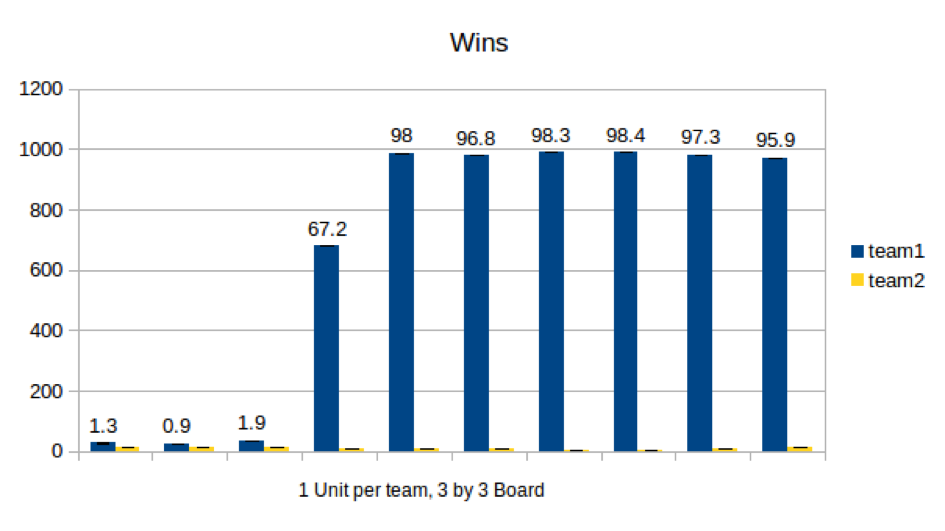
\includegraphics[width= 9 cm,height= 16 cm,keepaspectratio]{1v1}}
%  \vspace{2.0cm}
  
\end{minipage}
\caption{One unit in each team in a 3 by 3 board}
\label{fig:1v1}
%
\end{figure}

The first experiment sets both team sizes to 1 unit each with a board size of 3 by 3 and runs 10000 games. With only 1 unit per team, no information can be shared between units so each algorithm should perform the same in terms of learning. WIth a board size of 3 by 3, both units are able to reach each other and kill the enemy within a single turn. As a unit learns from game to game it should explore most, if not all, of the state-action space and eventually the action of killing an enemy will be discovered and reinforced positively. After enough runs, the team who takes the first turn should win every time since it will have positively reinforced the action of killing the enemy within a single turn. Looking at Figure~\ref{fig:1v1}, it is evident that one team was the clear overall winner. As you can see, during the first couple thousand games neither team was beating the other. Eventually, team 1 learned how to kill team 2. At this point, due to the bias nature of the game setup, team 1 fully learned how to win almost every game.
%Looking at Table~\ref{tab:SanityCheck}, it is evident that one team was the clear overall winner. It is also evident that on average the number of turns taken for either team to win is only a single turn, or close to it.



The second experiment sets both team sizes to $3$ on a board of size $5$ by $8$, and runs for $10000$ games. This is a larger board and both teams are bigger, giving each algorithm room to learn differently. With more than $1$ unit per team, sharing becomes a factor as well so here we expect to see Oracle outperform both Independent and Cooperative. We also expect to see Cooperative outperform Independent. Over 10000 games, we see in Figure-~\ref{fig:CvO} and Figure-~\ref{fig:IvO} that indeed oracle does win more often and with a higher score than the other two algorithms. Cooperative also outperforms Independent, but by an even slighter margin [Figure-~\ref{fig:IvC}]. As the win rate, and score are within small bounds when comparing one algorithm to another, we believe this leaves room for further improvement, discussed in section ~\ref{futurework}. The red curve in figure-\ref{fig:IvC}, figure-\ref{fig:CvO}, figure-\ref{fig:IvO} is reflecting the learning rate of the agents.
%Table~\ref{tab:TrueExperiment} that indeed oracle does win more often and with a higher score than the other two algorithms. Cooperative also outperforms Independent in score and turns taken to win, but by an even slighter margin. As the win rate, score, and turn average are within small bounds when comparing one algorithm to another, we believe this leaves room for further improvement, discussed in section ~\ref{futurework}

\begin{figure}[htb]

\begin{minipage}[b]{1.0\linewidth}
  \centering
  \centerline{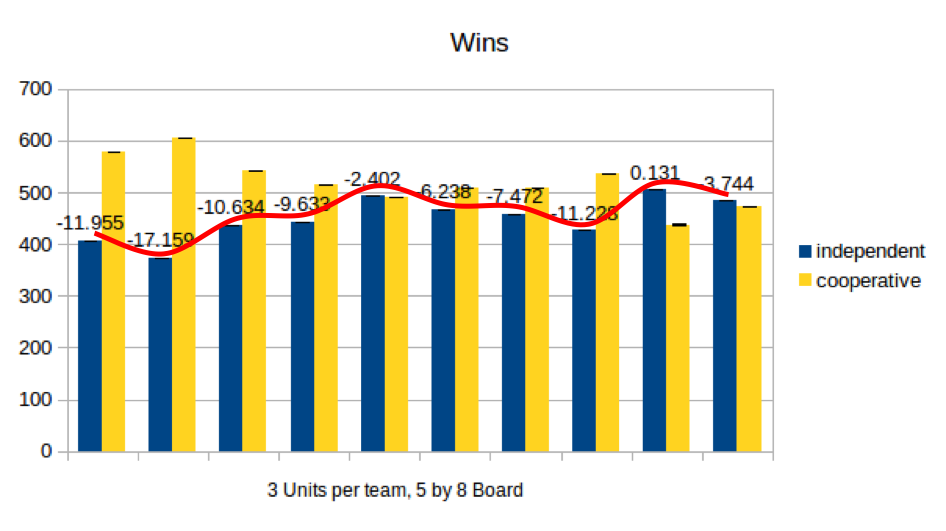
\includegraphics[width= 9 cm,height= 16 cm,keepaspectratio]{IvC}}
%  \vspace{2.0cm}
  \caption{Independent vs Cooperative teams with 3 units in each team in a 5 by 8 board}
\label{fig:IvC}
\end{minipage}
\end{figure}

\begin{figure}[htb]
\begin{minipage}[b]{1.0\linewidth}
  \centering
  \centerline{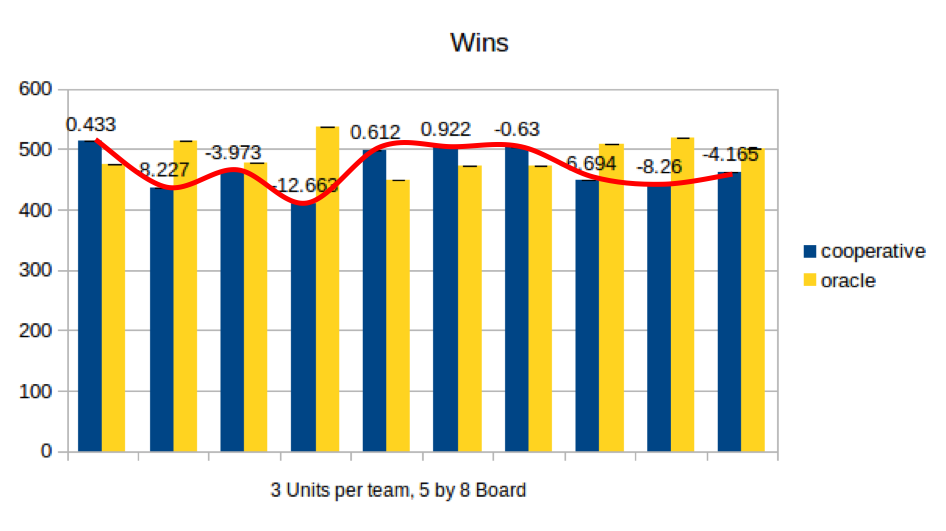
\includegraphics[width= 9 cm,height= 16 cm,keepaspectratio]{CvO}}
%  \vspace{2.0cm}
  \caption{Cooperative vs Oracle teams with 3 units in each team in a 5 by 8 board}
\label{fig:CvO}
\end{minipage}
\end{figure}

\begin{figure}[htb]
\begin{minipage}[b]{1.0\linewidth}
  \centering
  \centerline{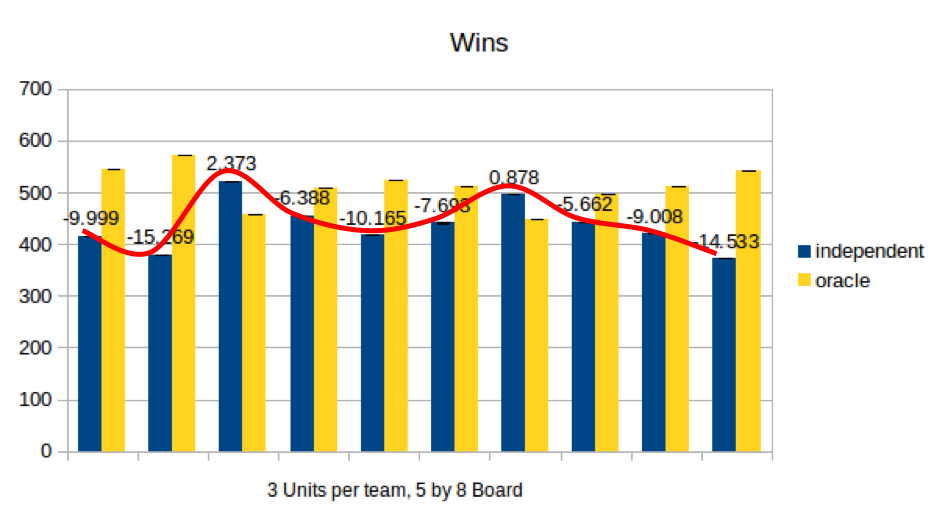
\includegraphics[width= 9 cm,height= 16 cm,keepaspectratio]{IvO}}
%  \vspace{2.0cm}
  \caption{Independent vs Oracle teams with 3 units in each team in a 5 by 8 board}
\label{fig:IvO}
\end{minipage}

%
\end{figure}


%that indeed Oracle does win more often and with a higher score against the other two algorithms. Cooperative also shows to outperform Independent in score and turns taken to win. The win rate, score, and turn average are with small bounds when comparing one algorithm to another and we believe this leaves room for further improvement, discussed in~\ref{futurework}.

%%%% basing on the number of games, show a table to compare the learning

\iffalse
\begin{table}[htbp] \hspace{-1cm}
\centering
\begin{tabular}{c|c|c|c}
 & Wins & Score & Turns  \\ \hline
Oracle & 0.82 (0.003) & 80.14 (0.33) & 2.26 (0.005)\\
vs. Independent & 0.17 (0.003) & 15.42 (0.33) & 1.96 (0.003)\\ \hline
Independent & 0.02 (0.001) & 1.44 (0.13) & 1 (0)\\
vs. Cooperative & 0.97 (0.001) & 96.55 (0.13) & 1 (0)\\ \hline
Cooperative & 0.02 (0.001) & 1.25 (0.13) & 1 (0) \\
vs. Oracle & 0.97 (0.001) & 96.74 (0.13) & 1 (0)
\end{tabular}
\caption{Team Size: 1, Board Size: 3 x 3, 50000 games. Results are read as: value (+/- confidence in value)}
\label{tab:SanityCheck}
\end{table}



\begin{table}[htbp] \hspace{-1cm}
\centering
\begin{tabular}{c|c|c|c}
 & Wins & Score & Turns  \\ \hline
Oracle & 0.54 (0.009) & 65.39 (0.58) & 9.75 (0.16)\\
vs. Independent & 0.45 (0.009) & 58.23 (0.61) & 10.94 (0.19)\\ \hline
Independent & 0.5 (0.009) & 62.41 (0.59) & 10.61 (0.15)\\
vs. Cooperative & 0.5 (0.009) & 65.56 (0.55) & 9.67 (0.15)\\ \hline
Cooperative & 0.48 (0.009) & 63.33 (0.57) & 10.13 (0.15) \\
vs. Oracle & 0.51 (0.009) & 62.55 (0.59) & 11.17 (0.16)
\end{tabular}
\caption{Team Size: 3, Board Size: 6 x 9, 10000 games. Results are read as: value (+/- confidence in value)}
\label{tab:TrueExperiment}
\end{table}

\vspace{-.5 cm}
\fi
\section{Future Work} \label{futurework}


The performance increase obtained by information sharing in our results was modest. We have identified a number of ways in which the algorithms and game could be modified to potentially increase performance by information sharing. The message sharing could be modified to include sharing percepts and events. In this context, that could mean allowing units to know the locations of their allied units beyond their line of sight and the locations of enemy units seen by their allies. The units could also share not just new Q-Values, but every state-action-reward tuple so that allied units can update their Q-Values with this information even after a given state-action pair has been explored once. Sharing can also be extended from only sharing with allies to sharing with yourself as well. It is possible to find the degree of similarity between a unit's current state and different states a unit has already visited and predict the best next action based on the actions taken in similar previous states. The agents could also be modified to have a commander unit, which would make decisions for all of its allied units to help the team as a whole.
 \endinput
 
 %independent :: may have a commander
 %cooperative :: may share other 2 formats of message
 %coopeartive :: share state with self
\section{Conclusion}
From the experiments, it is observed that Oracle, where there is unlimited message sharing, has the best performance. However this can never be applied in a real time scenario where there can only be limited message sharing among agents acting in any field (e.g. a battlefield). Also, we have seen that the performance is poor in the case of independent agents, which implies that message sharing is important in a multi-agent environment. From our results, we can also see that the difference in performance between the MARL AI algorithms is negligable leaving room for further development and future improvement.

\vspace{-.2 cm}
 \endinput

\bibliographystyle{abbrv}
\bibliography{bib/references}

\section{Reviews} The reviews and responses are listed below. Since the section number in the final version of the paper is different from the initial version, we added the name of the section which the reviewer mentioned in brackets.
%is Since we need an extra page describing how we incorporate the reviews into the paper we can just address them one at a time and comment the changes made here.

\subsection{Review 1}
\begin{enumerate}
\item Please include more related work to explain the message sharing (e.g. facts and events)\\
{\it Response : }Message sharing is explained in more detail in the later section-\ref{Oracle_Agent}, \ref{Coop_Agent}, \ref{Independent_Agent}.

\item Although introduced in details later, could you explain action, state and rewards in more details in section 3.1 and 3.2 (Reinforcement learning and multiple agent learning) maybe with some examples.\\
{\it Response : }We added some additional detail to section-\ref{RL}.
\item I suppose some parameters for the variables in Equation 1 are not shown explicitly, e.g. 'r' has parameters 'state' and 'action'.\\
{\it Response : }We added explanations for each variable in the equation.
\item Maybe you could introduce each kind of agent first and compare them in a new section\\
{\it Response : }We briefly added a section-\ref{AgentDesign}
\item For the result, could you run examples with larger board size and team size?\\
{\it Response : }We include results for 5x8. Results for larger sizes perform similarly but take longer, so we opt to not include these in the paper due to space limitations.
\end{enumerate}

\subsection{Review 2}
\begin{enumerate}
\item In Equation (1),neither the description nor the intuitive reasoning behind the parameter 'α' is not given. From the context, I am to understand that it is a learning rate similar to the stochastic gradient descent method. It would be nice to clarify the same in this proposal.  %added the explanation for alpha
\\{\it Response : }See review 1, point 3.

\item The section about the usage of Q-Values in the overall algorithm is a little handwavy - the precise way how it determines the overall running of the algorithm is not mentioned in sections 3.3 (Q-Learning) which manifests in an unclear understanding of section 4.1 (Oracle Agent) - The sentence "On the other hand if the black circled units are controlled by oracle agent then the agent will choose either unit-1 or unit-2 based on their Q-values to attack unit-A" is hard to comprehend when the exact role of Q-Values if not known. 
\\{\it Response : } We added more detail to section-\ref{QL}, and the section quoted above was completely removed from the paper as we took a different direction with our message sharing implementation.


\item I believe that there is a discrepancy in the results for table 1. In the event that there are 2 teams with 1 member each where the game ends in a single turn - both independent and oracle play should produce the same result (since they are the same in this particular case). However it seems from the table that there is an imbalance in the two. That is the ratio is 0.82:0.17 whereas it should have been 0.5 to 0.5 since the two are essentially equivalent. (This result is surprisingly reflected in table 2). It may be a problem in my understanding of the table semantics however it would behoove the authors to provide clarity in the said aspect in the final draft. 
\\{\it Response : }New figures are added instead of the tables in the revised version to clarify this confusion.


\item The authors don't provide any analysis for the convergence of the gameplay algorithm. More specifically, I am curious if there can be any situations where there is a deadlock in the game play (I can envision a situation where there are two agents left in a board and one agent plays the game offensively while the other agent plays defensively essentially producing a "cat-mouse" situation which can extend the game for a large turns - such a situation while uncommon may occur). I believe that the parameters in the Q-Value computation can help in determining if such an analysis exists or not. 
\\{\it Response : } If by convergence, the reviewer meant when we should stop training our algorithm to start testing with. We agreed that there is no true convergence since agents learn indefinitely. As an evaluation, we show that there is a point in which learning for an agent in a particular game setup will stop making significant process.

\item I believe that section 4.3 can benefit from some clarity. The two parameters which are crucial to correct information sharing - " limited to only sharing with a set number of allies and only specifically requested information. " It is not clear how the first parameters will be determined. Also not clear is how the agents will learn the information to be requested - is it a part of the learning or will it be fixed. In the former case, the ML complexity of the algorithm increases while in the latter case, it will suffer from slow learning rate since it may keep on optimization over a set of values on which we already have sufficient information. 
\\{\it Response : } The number of allies to share information with is random. So when sharing, we choose a random subset of allies to share with. The actual process of sharing information with allies happens by sharing Q-Values after an action is taken. Given a set of allies to share with, if a chosen ally has also taken the same action as some point the Q-Value for the unit and the ally are averaged together. In addition to averaging Q-Values, the value function will also average the Q-Values of the next state. The same subset of allies will be chosen to share with and if a chosen ally has also taken the same next action at some point the Q-Value for the unit and the ally used to calculate the Value Function will average together.

\end{enumerate}

\subsection{Review 3}
\begin{enumerate}
\item would suggest moving the description of the game that is being played earlier in the paper.
\\{\it Response : }We restructured the paper to introduce the game earlier.

\item I was confused on the specific type of game being played when I started reading.
I was confused about the results. Why, in the case of a single unit, would one algorithm outperform another. 
\\{\it Response : } In case of single unit, the point is that there is no difference in the performance of different AI agents. Whichever team starts first wins.

\item Even in section 5 you mention that no sharing is being done, so each algorithm should perform the same, but Table 1 shows differently. Could you address this or clarify this?
\\{\it Response : } Corrected this and replaced the table with our new results Fig-\ref{fig:1v1}.

\item In Table 2 the results between the algorithms seem close enough to maybe be statistical error. How are you sure that one algorithm outperforms another?
\\{\it Response : }We changed the presentation of results to emphasize that the differences in performance are not, in fact, that strong.

\item I would like to see some questions asked at the end about generalizing. Could this technique work for a less contrived game, like a modern turn based or RTS game? 
\\{\it Response : }The different AI make decision based on different states, the possible actions from those states, and what kind of reward a unit should receive for taking an action. If states, actions, and rewards are properly defined for each game then the algorithm simply needs a new state as an input and will provide an action to take.


\item Does cooperative passing provide a better experience for a user, or do they not care?
\\{\it Response : }for 1 user there is no difference

\item I noticed a small typo in section 2(BACKGROUND AND RELATED WORK): messages passing
\\{\it Response : }Typo corrected
\item All in all I think this is a good and interesting paper.
\end{enumerate}

\subsection{Review 4}
\begin{enumerate}
\item The biggest problem is that you didn't describe Cooperative Agent clearly in section 4.3, while Cooperative Agent is supposed to be your key innovation in this paper. You may add some explanation of how the Cooperative Agent incorporates (uses) the received information and in what ways it is different from the Oracle Agent.\\
{\it Response : }Added the explanation for cooperative agent in section-\ref{Coop_Agent}.

\item It is not appropriate to say that Reinforcement Learning is a form of Unsupervised Learning. The "prior knowledge" in a Reinforcement Learning system is the rewards, or the rewards generating system. A more rational division of  learning algorithms should be Supervised Learning, Unsupervised Learning and Reinforcement Learning.\\
{\it Response : }We changed how we introduce and describe Reinforcement Learning.

\item In your first experiment, where there is only one unit, the result shows a clear relationship that Oracle Agent outperforms Cooperative Agent, and Cooperative Agent is better than Independent Agent. How do you explain this? If it is totally because of the order that who runs first, you may start from a randomly selected agent at each episode.\\
{\it Response : }See review 3, point 2

\item The order of your bibliography is confusing. For example, the number of your bibliography jumps from "[1]" to "[6]", and then jumps back to "[4]" in your introduction and background section.\\
{\it Response : }We use abbrv format, which is an acceptable bibliography format.

\item The explanation to Formula 1 in your paper is correct in general. However, if you are familiar with the mathematical derivation of  the Markov Decision Process, it may not be appropriate to use "V" as the  optimal Q value, since "V" is commonly used to denote the state-value function. In addition, the explanation of "V" in your paper should be more accurate. In another word, you should tell explicitly for which state "V" is the maximal Q-value. Perhaps it is helpful for you to take a deeper study of the mathematical foundation of Reinforcement Learning and Bellman Equation.\\
{\it Response : }See review 1, point 3

\item The keywords you selected may be inappropriate, since the concept of one keyword may belong to another one.\\
{\it Response : }Conference papers also have some overlapping keywords, so we think this is fine

\item Some prior art you mentioned may not be directly relevant to the topic of this paper, for example, the multi-agent foraging example in the background section.\\
{\it Response : }It is added as a concrete example of Multi Agent Systems, especially demonstrating a situation where multiple agents may have limited bandwidth with which to share information.
\end{enumerate}


\end{document}
